\documentclass[tikz,border=6pt]{standalone}
\usepackage{pgfplots}
\pgfplotsset{compat=1.18}
\begin{document}
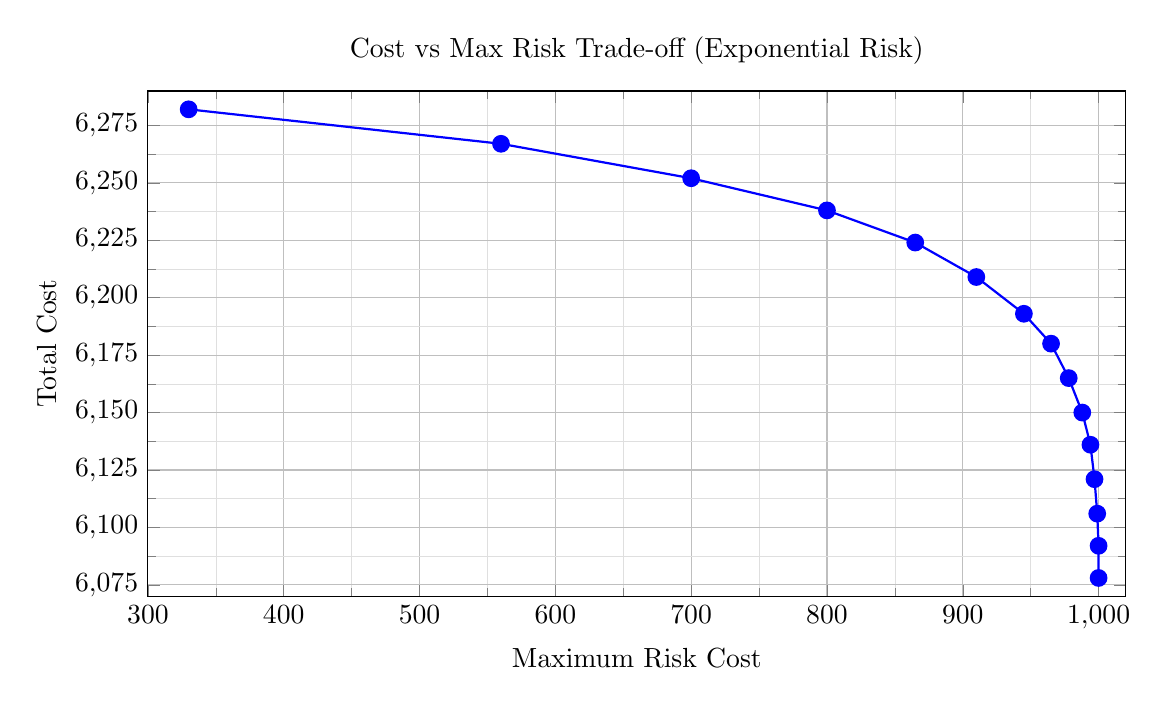
\begin{tikzpicture}
\begin{axis}[
    width=14cm,
    height=8cm,
    title={Cost vs Max Risk Trade-off (Exponential Risk)},
    xlabel={Maximum Risk Cost},
    ylabel={Total Cost},
    xmin=300, xmax=1020,
    ymin=6070, ymax=6290,
    xtick={300,400,500,600,700,800,900,1000},
    ytick={6075,6100,6125,6150,6175,6200,6225,6250,6275},
    grid=both,
    major grid style={line width=0.4pt, draw=gray!50},
    minor grid style={line width=0.2pt, draw=gray!25},
    minor tick num=1,
]
% Approximate points reconstructed from the image
\addplot[
    thick,
    blue,
    mark=*,
    mark size=2.8pt,
]
coordinates {
    (330,6282)
    (560,6267)
    (700,6252)
    (800,6238)
    (865,6224)
    (910,6209)
    (945,6193)
    (965,6180)
    (978,6165)
    (988,6150)
    (994,6136)
    (997,6121)
    (999,6106)
    (1000,6092)
    (1000,6078)
};
\end{axis}
\end{tikzpicture}
\end{document}
